\documentclass[journal,12pt,twocolumn]{IEEEtran}
\usepackage[utf8]{inputenc}
\usepackage{amsmath}
\usepackage{graphicx}
\usepackage[english]{babel}
\newtheorem{proof}{PROOF}
\usepackage{hyperref}
\usepackage{tcolorbox}
\urlstyle{same}
\title{Assignment  }
\author{Harshal Verma\\
AI21MTECH02003}
\date{April 2021}
\begin{document}
\maketitle
\section{GATE EC 8}
Problem: Consider a dice with the property that the probability of a face with n dots showing up is proportional to n. The probability of the face with three dots showing up is ?\\
\\
\textbf{Solution}: Given that the dice with the
 property that the probability of a face with n dots showing up is proportional to n , let the proportionality constant be 'c' .\\
 $\Pr(N)$ is proportional to n
 where n=\{1, 2, 3, 4, 5, 6\} is random variable.\\
Then $\Pr(n) = n \times c $, tabulating the outcomes : 
\\
\begin{center}
\begin{tabular}{ |c | c | c | c | c | c | c |}
\hline
n     & 1 & 2 & 3 & 4 & 5 & 6 \\
\hline
$\Pr(N = n ) = n \times c$ & 1c & 2c&3c &4c & 5c & 6c\\
\hline
\end{tabular}
\end{center}
\smallskip
As the sum of all probability is equal to 1\\
\begin{align*}
\Sigma_{N=n} \Pr(N) &= 1\\
c + 2c + 3c + 4c + 5c + 6c &= 1\\
21c &= 1\\
c &= \frac{1}{21}\\
\end{align*}
\smallskip
\text{The probability of three dots showing up is 3c} \\
\text{Giving the probability to be:}\\
\begin{align*}
\Pr(N=3) &= 3 \times c\\
&= 3\times\frac{1}{21}\\
&= \frac{3}{21}\\
&= \frac{1}{7}\\
&= 0.1428   
\end{align*}
The probability of getting a face with three dots showing up is 0.1428
\samllskip
\begin{figure}[htp]
    \centering
    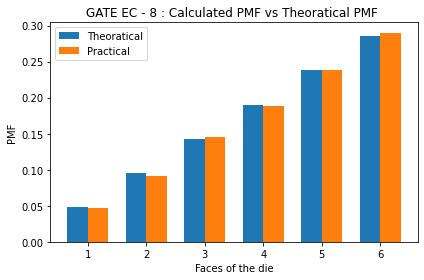
\includegraphics[width=10cm]{Assignment_9_1.png}
    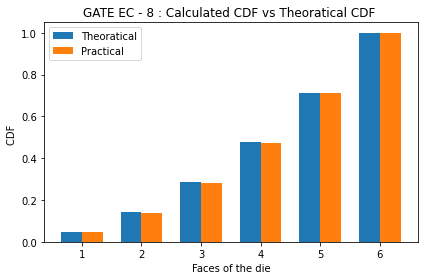
\includegraphics[width=10cm]{Assignment_9_2.png}
    \label{fig :plot}
\end{figure}
\smallskip
\begin{tcolorbox}
Code source: \url{https://github.com/harshal9876/AI5002/blob/main/Assignment_9/Codes/Assignment_9.py} \\
LaTex code :
\url{https://github.com/harshal9876/AI5002/blob/main/Assignment_9/Assignment_9.tex}
\end{tcolorbox}
\vfill
\end{document}



